\chapter{DISEÑO DE LA SOLUCIÓN}

\section{Antecedentes Teóricos}

La construcción de un observatorio de demanda laboral automatizado requiere la integración de múltiples técnicas del estado del arte en procesamiento de lenguaje natural, aprendizaje automático y análisis de datos. Esta sección presenta los fundamentos teóricos que sustentan las decisiones de diseño del sistema, estableciendo el marco conceptual sobre el cual se construyó la solución propuesta. El análisis comparativo de estas técnicas, junto con su evaluación empírica en el contexto del español latinoamericano, proporciona la base para las decisiones arquitectónicas presentadas en secciones posteriores.

\subsection{Técnicas de Extracción de Información}

La extracción de información (IE) es el proceso de identificar y extraer automáticamente datos estructurados a partir de fuentes no estructuradas \cite{sarawagi2008}. En el dominio del análisis de demanda laboral, el objetivo específico es identificar habilidades, tecnologías y competencias mencionadas en ofertas de empleo publicadas en portales web. Las técnicas modernas de extracción se clasifican en tres categorías principales según su nivel de dependencia de conocimiento previo y capacidad de inferencia semántica.

\subsubsection{Reconocimiento de Entidades Nombradas (NER)}

El Reconocimiento de Entidades Nombradas es una tarea fundamental de NLP que consiste en localizar y clasificar entidades en texto dentro de categorías predefinidas \cite{nadeau2007}. Los sistemas NER modernos se basan en modelos de aprendizaje supervisado, particularmente arquitecturas basadas en transformers \cite{devlin2019}. Para el dominio de habilidades técnicas, NER presenta ventajas significativas: alta precisión para entidades conocidas (>90\%), contextualización bidireccional para desambiguación, y eficiencia computacional con latencias de milisegundos por documento \cite{zhang2018}. Sin embargo, enfrenta limitaciones críticas: dependencia del vocabulario de entrenamiento, baja cobertura en dominios especializados, y la incapacidad de inferir habilidades implícitas no mencionadas explícitamente en el texto \cite{canete2020}.

En este proyecto se adoptó un enfoque híbrido que combina el modelo base \texttt{es\_core\_news\_lg} de spaCy con un EntityRuler personalizado poblado con la taxonomía ESCO (13,000+ habilidades), permitiendo reconocimiento directo de terminología técnica no presente en el modelo pre-entrenado \cite{decorte2021}.

\subsubsection{Extracción basada en Expresiones Regulares}

Las expresiones regulares (regex) son patrones de búsqueda basados en lenguajes formales que permiten identificar secuencias de caracteres con estructuras específicas \cite{friedl2006}. En el contexto de extracción de habilidades técnicas, regex es particularmente efectiva para tecnologías con nomenclaturas estandarizadas: versiones numeradas (``Python 3.x'', ``Java 8+''), frameworks con sufijos convencionales (``.js'', ``SQL''), y acrónimos técnicos (``REST API'', ``CI/CD''). Sus ventajas incluyen precisión del 100\% en patrones bien definidos, transparencia y auditabilidad, velocidad extrema (microsegundos por documento), y ausencia de requisitos de entrenamiento. Las limitaciones principales son fragilidad ante variaciones ortográficas, mantenimiento manual intensivo, y ausencia de comprensión contextual \cite{chiticariu2013}.

\subsubsection{Extracción basada en Modelos de Lenguaje Grandes (LLMs)}

Los Large Language Models representan un cambio de paradigma en NLP, basándose en arquitecturas transformer pre-entrenadas sobre corpus masivos mediante objetivos de modelado de lenguaje \cite{brown2020, touvron2023}. A diferencia de NER y regex, los LLMs poseen capacidades de razonamiento contextual que permiten: inferencia de habilidades implícitas (deducir que un ``Científico de Datos'' requiere estadística y Python aunque no se mencione), normalización semántica automática (identificar que ``React'', ``React.js'' y ``ReactJS'' son equivalentes), desambiguación contextual, adaptación al lenguaje informal y ``Spanglish'', y razonamiento explicable mediante prompt engineering \cite{zhang2023, wei2023, vilares2016}.

Sin embargo, presentan limitaciones significativas: latencia 100-1000x mayor que NER (segundos vs. milisegundos), no-determinismo con temperatura $>$ 0, alucinaciones que generan habilidades incorrectas, alto costo computacional (GPUs o APIs de pago), y sesgo lingüístico hacia el inglés con rendimiento degradado en español técnico \cite{elazar2023, ji2023, banon2020}.

\subsubsection{Justificación del Enfoque Dual}

La Tabla \ref{tab:comparacion-tecnicas-extraccion} presenta una comparación sistemática de las tres técnicas según criterios relevantes para el observatorio.

\begin{table}[H]
\centering
\caption{Comparación de Técnicas de Extracción de Habilidades}
\label{tab:comparacion-tecnicas-extraccion}
\begin{tabular}{|p{3cm}|p{3.5cm}|p{3.5cm}|p{3.5cm}|}
\hline
\textbf{Criterio} & \textbf{NER} & \textbf{Regex} & \textbf{LLMs} \\
\hline
Precisión (explícitas) & Alta (85-95\%) & Muy alta (95-100\%) & Media-alta (80-90\%) \\
\hline
Recall (cobertura) & Media (60-75\%) & Baja (40-60\%) & Alta (75-90\%) \\
\hline
Habilidades implícitas & No soportado & No soportado & Soportado \\
\hline
Latencia & Baja (5-20 ms) & Muy baja (<1 ms) & Alta (2-10 s) \\
\hline
Costo computacional & Bajo (CPU) & Muy bajo (CPU) & Alto (GPU/API) \\
\hline
Mantenimiento & Moderado & Alto & Bajo \\
\hline
Español LATAM & Medio & Alto & Variable \\
\hline
\end{tabular}
\end{table}

Dado que ninguna técnica individual satisface todos los requisitos, se adoptó una \textbf{arquitectura dual de pipelines paralelos}: \textbf{Pipeline A} (NER + Regex + ESCO) optimizado para alta precisión y baja latencia, procesando el 100\% de las ofertas; y \textbf{Pipeline B} (LLMs) para enriquecimiento semántico y detección de habilidades implícitas en un subconjunto estratégico. Esta arquitectura permite evaluación empírica comparativa donde Pipeline A sirve como control de alta precisión y Pipeline B como tratamiento de alta cobertura \cite{li2023}.

\subsection{Modelos de Lenguaje Grandes}

Los Large Language Models se basan en arquitecturas transformer que utilizan mecanismos de auto-atención para capturar dependencias contextuales de largo alcance \cite{vaswani2017}. El pre-entrenamiento mediante modelado de lenguaje causal les permite adquirir capacidades de razonamiento y comprensión lingüística sin requerir datasets anotados específicos del dominio \cite{brown2020, wei2022emergent}.

Para el Pipeline B del observatorio, se identificaron cuatro familias de LLMs como candidatos, evaluados según criterios de costo, rendimiento, soporte multilingüe y capacidad de despliegue local.

\subsubsection{Candidatos Evaluados}

\textbf{GPT-4 y GPT-3.5 (OpenAI)} representan el estado del arte con F1-scores de 0.68 y 0.62 en extracción de habilidades en inglés respectivamente \cite{openai2023gpt4, zhang2023}. Ofrecen soporte multilingüe robusto, despliegue simplificado mediante API REST, y function calling nativo para salidas estructuradas. Sin embargo, el costo es elevado (\$255 y \$8.5 respectivamente para 23K jobs), requieren conectividad constante con latencias variables (1-10s), y son black-box sin posibilidad de fine-tuning.

\textbf{Mistral 7B Instruct} es un modelo open-source de 7.3B parámetros que utiliza Grouped-Query Attention y Sliding Window Attention para mejorar eficiencia \cite{jiang2023mistral}. Logra F1=0.58 en español superando a LLaMA 2 13B. Sus ventajas incluyen eficiencia de inferencia con cuantización Q4 (4-5 GB VRAM), licencia Apache 2.0, y costo cero. Las limitaciones son pre-entrenamiento principalmente en inglés (70\% corpus, 15\% español), vocabulario técnico limitado, y latencia de 3-7s en GPU.

\textbf{LLaMA 3 8B Instruct} (Meta AI) está entrenado sobre 15 billones de tokens con vocabulario expandido de 128K tokens \cite{touvron2023llama3}. Logra F1=0.64 en extracción de habilidades, el mejor balance para despliegue local \cite{nguyen2024}. Ventajas: corpus de pre-entrenamiento con 5\% español de alta calidad, tokenización eficiente (1.3 tokens/palabra vs 1.8 en Mistral), fine-tuning instruccional con 10M ejemplos, y latencia competitiva (2-5s con Q4). Limitaciones: requisitos de memoria superiores (8-10 GB VRAM) y licencia restrictiva para aplicaciones con $>$700M usuarios activos mensuales.

La Tabla \ref{tab:comparacion-llms} resume la comparación cuantitativa.

\begin{table}[H]
\centering
\caption{Comparación de Large Language Models para Extracción de Habilidades}
\label{tab:comparacion-llms}
\begin{tabular}{|p{2.5cm}|p{2cm}|p{2cm}|p{2cm}|p{2cm}|}
\hline
\textbf{Criterio} & \textbf{GPT-3.5} & \textbf{GPT-4} & \textbf{Mistral 7B} & \textbf{LLaMA 3 8B} \\
\hline
Parámetros & 175B & 1.76T (MoE) & 7.3B & 8B \\
\hline
F1 (Español) & 0.59 & 0.65 & 0.52 & 0.61 \\
\hline
Latencia (GPU) & 2-5s & 3-8s & 3-7s & 2-5s \\
\hline
Costo (23K jobs) & \$8.5 & \$255 & \$0 & \$0 \\
\hline
VRAM (Q4) & N/A (API) & N/A (API) & 4-5 GB & 8-10 GB \\
\hline
Despliegue & Cloud API & Cloud API & Local & Local \\
\hline
Licencia & Propietaria & Propietaria & Apache 2.0 & LLaMA 3 CL \\
\hline
Tokens/palabra & 1.5 & 1.5 & 1.8 & 1.3 \\
\hline
\end{tabular}
\end{table}

\subsubsection{Selección y Justificación}

Se seleccionó \textbf{LLaMA 3 8B Instruct} fundamentado en: (1) Balance rendimiento-eficiencia: F1=0.61 en español con 8B parámetros, acercándose a GPT-3.5 (F1=0.59) a costo cero; (2) Despliegue local: elimina dependencias de APIs, costos recurrentes y garantiza privacidad de datos laborales sensibles; (3) Tokenización eficiente: vocabulario de 128K tokens logra 1.3 tokens/palabra preservando mejor terminología técnica compuesta; (4) Licencia permisiva para aplicaciones académicas ($<$700M MAU). Se planea una evaluación experimental comparativa donde GPT-3.5, GPT-4, Mistral 7B y LLaMA 3 procesarán 300 jobs anotados manualmente, permitiendo validación empírica mediante métricas de Precision, Recall y F1-score.

\subsection{Embeddings Semánticos y Búsqueda de Similitud}

Los embeddings semánticos son representaciones vectoriales densas que capturan relaciones semánticas mediante proximidad en espacios de alta dimensionalidad \cite{mikolov2013}. A diferencia de representaciones dispersas (TF-IDF), los embeddings permiten que términos semánticamente relacionados tengan vectores cercanos incluso sin compartir palabras exactas \cite{reimers2019}.

En el observatorio, los embeddings cumplen dos roles: (1) normalización de habilidades extraídas contra taxonomía ESCO mediante búsqueda de similitud coseno, y (2) agrupamiento de habilidades para descubrir perfiles emergentes. El modelo \texttt{intfloat/multilingual-e5-base} fue seleccionado por su soporte multilingüe nativo (768D, 100 idiomas, entrenado con contrastive learning) \cite{wang2024}, normalización L2 integrada, tamaño compacto (278M parámetros ejecutables en CPU $<$100ms/batch), y licencia MIT.

\subsubsection{Limitaciones Empíricas y Decisión Arquitectónica}

La evaluación experimental con 15 habilidades técnicas agregadas manualmente a ESCO reveló limitaciones críticas del modelo E5. Con threshold de similitud coseno = 0.75, se obtuvo tasa de matches correctos de 6.7\% (1/15) y falsos positivos de 93.3\% (14/15). Ejemplos: ``React'' $\rightarrow$ ``neoplasia'' (0.828), ``Docker'' $\rightarrow$ ``Facebook'' (0.825), ``Machine Learning'' $\rightarrow$ ``gas natural'' (0.825). El análisis de causa raíz identificó tres factores: entrenamiento en lenguaje natural vs. vocabulario técnico, confusión entre brand names y palabras comunes, y contaminación del espacio vectorial por 13,939 habilidades ESCO de dominios no técnicos.

La evaluación de thresholds demostró que no existe un valor que balancee precision y recall: thresholds bajos ($<$0.80) generan falsos positivos críticos, mientras que thresholds altos ($\geq$0.85) excluyen matches exactos. Con base en esta evidencia, se tomó la decisión de \textbf{deshabilitar la capa de búsqueda semántica (Layer 3)}, operando el sistema con estrategia de dos capas: \textbf{Layer 1 (Exact Match)} mediante búsqueda SQL con confidence = 1.00, y \textbf{Layer 2 (Fuzzy Match)} con threshold = 0.85 para capturar variantes ortográficas.

Para búsqueda de similitud en clustering, se adoptó \textbf{FAISS (Facebook AI Similarity Search)} con índice IndexFlatIP (exact search con inner product). FAISS demostró performance superior: 30,147 queries/segundo, latencia 0.033ms por query, speedup 25x sobre PostgreSQL pgvector, superando ampliamente el objetivo de diseño (100 q/s) por un margen de 301x \cite{johnson2019}.

\subsection{Técnicas de Clustering No Supervisado}

El descubrimiento de perfiles laborales emergentes requiere técnicas de clustering que operen sin conocimiento previo de las categorías objetivo. El sistema integra dos algoritmos complementarios para proyección dimensional y agrupamiento basado en densidad.

\subsubsection{UMAP (Uniform Manifold Approximation and Projection)}

UMAP es un algoritmo de reducción dimensional no lineal fundamentado en teoría de variedades Riemannianas y topología algebraica \cite{mcinnes2018umap}. A diferencia de t-SNE, UMAP preserva tanto estructura local (relaciones entre vecinos cercanos) como estructura global (relaciones entre clústeres distantes), fundamental para análisis de mercado laboral donde se requiere mantener jerarquías de habilidades. Los parámetros clave son: \texttt{n\_neighbors=15} (balance entre estructura local y global), \texttt{min\_dist=0.1} (compactación de puntos cercanos), y \texttt{metric='cosine'} (métrica de similitud apropiada para embeddings normalizados). UMAP reduce vectores de 768 dimensiones a 2-3 dimensiones visualizables manteniendo propiedades semánticas.

\subsubsection{HDBSCAN (Hierarchical Density-Based Spatial Clustering)}

HDBSCAN es un algoritmo de clustering jerárquico basado en densidad que extiende DBSCAN mediante construcción de un árbol de conectividad mínima \cite{campello2013}. Sus ventajas clave para este dominio incluyen: no requiere especificar el número de clústeres k (crítico cuando el número de perfiles emergentes es desconocido), identifica ruido automáticamente (habilidades atípicas o errores de extracción), maneja clústeres de densidades variables (perfiles nicho vs. mainstream), y proporciona jerarquía que permite análisis multinivel (familias de roles $\rightarrow$ roles específicos). Parámetros: \texttt{min\_cluster\_size=5} (tamaño mínimo de clúster válido), \texttt{min\_samples=3} (puntos mínimos para núcleo de densidad), y \texttt{metric='euclidean'} (post-reducción dimensional con UMAP).

\subsection{Taxonomías de Habilidades Laborales}

La normalización de habilidades extraídas requiere una taxonomía de referencia robusta, multilingüe y mantenida activamente. Se evaluaron tres alternativas principales.

\subsubsection{Alternativas Consideradas}

\textbf{O*NET (Occupational Information Network)} es la taxonomía del Departamento de Trabajo de EE.UU. con 1,000+ ocupaciones y 20,000+ habilidades. Ventajas: altamente estructurada con relaciones jerárquicas, actualización periódica, y datos salariales asociados. Limitaciones: enfoque en mercado estadounidense, escasa cobertura de tecnologías emergentes, y ausencia de soporte multilingüe nativo.

\textbf{ESCO (European Skills, Competences, Qualifications and Occupations)} es la taxonomía oficial de la Unión Europea con 13,000+ habilidades, 3,000+ ocupaciones, y soporte para 27 idiomas \cite{decorte2021}. Ventajas: etiquetas nativas en español e inglés, cobertura amplia de habilidades tecnológicas, estructura ontológica con URIs únicos, y respaldo institucional de la Comisión Europea garantizando mantenimiento. Limitaciones: actualización menos frecuente que el mercado tecnológico (v1.1.0 data de 2016-2017), y menor cobertura de frameworks JavaScript modernos.

\textbf{Taxonomías propietarias} (LinkedIn Skills, Burning Glass Technologies): Ventajas: actualizadas con mayor frecuencia, cobertura de tecnologías emergentes. Limitaciones críticas: acceso mediante API de pago, licencias restrictivas, y falta de transparencia metodológica.

\subsubsection{Selección y Justificación}

Se seleccionó \textbf{ESCO v1.1.0} fundamentado en: (1) Soporte multilingüe nativo (español/inglés) eliminando necesidad de traducción automática; (2) Licencia Creative Commons BY 4.0 permitiendo uso académico y comercial sin restricciones; (3) Estructura ontológica con URIs persistentes facilitando integración con LLMs y sistemas de recomendación; (4) Cobertura de 13,000+ habilidades suficiente para establecer baseline, complementable con expansión manual de 174 habilidades técnicas modernas identificadas en el análisis exploratorio. La taxonomía se almacenó en PostgreSQL (tabla \texttt{esco\_skills}) con índices en \texttt{preferred\_label\_es}, \texttt{preferred\_label\_en} y \texttt{alt\_labels}, permitiendo búsquedas eficientes durante el matching.

\section{Pruebas de Modelos}

Esta sección presenta los resultados de las validaciones experimentales ejecutadas sobre el sistema de extracción y matching de habilidades. A diferencia de benchmarks teóricos sobre datasets en inglés, estas pruebas se realizaron con ofertas laborales reales de portales latinoamericanos, proporcionando evidencia empírica específica del dominio que fundamentó decisiones arquitectónicas clave presentadas en la sección anterior.

\subsection{Conjunto de Datos}

El dataset del observatorio se compone de ofertas laborales tecnológicas recolectadas mediante web scraping de seis portales principales en tres países: Computrabajo, Bumeran y ElEmpleo (Colombia); Computrabajo, Bumeran, InfoJobs y OCC Mundial (México); y Computrabajo, Bumeran y ZonaJobs (Argentina). Al momento de las pruebas de validación presentadas en esta sección, el corpus contenía 23,188 ofertas laborales únicas distribuidas como: Colombia 8,742 (37.7\%), México 9,856 (42.5\%), y Argentina 4,590 (19.8\%). Las ofertas abarcan el período de marzo a diciembre de 2024, con mayor concentración en los meses de agosto a octubre (58\% del total).

Cada oferta contiene los siguientes campos estructurados: \texttt{job\_id} (UUID único), \texttt{portal} (origen de la oferta), \texttt{country} (CO/MX/AR), \texttt{title} (título del cargo), \texttt{company} (empresa), \texttt{description} (descripción detallada del cargo), \texttt{requirements} (requisitos y habilidades), \texttt{salary\_raw} (rango salarial cuando disponible), \texttt{contract\_type} (tipo de contrato), \texttt{remote\_type} (modalidad presencial/remota/híbrida), \texttt{posted\_date} (fecha de publicación), y \texttt{content\_hash} (hash SHA-256 para deduplicación).

\subsection{Construcción del Conjunto de Datos}

\subsubsection{Proceso de Scraping}

La recolección de datos se ejecutó mediante Scrapy 2.11, un framework asíncrono de scraping en Python que permite procesamiento concurrente de múltiples requests. Para portales con contenido dinámico cargado mediante JavaScript (Bumeran, ZonaJobs), se integraron Selenium 4.15 y ChromeDriver para renderizado completo de páginas antes de la extracción. El proceso implementó técnicas de ``polite crawling'': delays adaptativos entre requests (2-5 segundos), rotación de user-agents, límites de concurrencia por dominio, y reintentos con backoff exponencial ante errores HTTP 429/503.

La deduplicación de ofertas se realizó mediante hashing SHA-256 del contenido normalizado (title + company + description limpiados), almacenando el hash en campo \texttt{content\_hash} con restricción UNIQUE en PostgreSQL. Esta estrategia evitó re-procesar ofertas republicadas por portales múltiples o reposteadas por el mismo portal.

\subsubsection{Limpieza y Normalización}

Las ofertas extraídas presentaron variabilidad significativa en formato y calidad. Se aplicó un pipeline de limpieza: eliminación de caracteres HTML residuales (\texttt{<br>}, \texttt{\&nbsp;}), normalización de espacios múltiples y saltos de línea, conversión de encoding a UTF-8, y extracción de texto plano de campos con formato rich text. Los disclaimers legales (equal opportunity statements, privacy policies) se identificaron mediante patrones regex y se separaron en metadatos sin afectar el análisis de habilidades.

\subsection{Validación de Técnicas de Extracción (Pipeline A)}

Se evaluó el rendimiento de los dos métodos del Pipeline A (Regex y NER) sobre 10 ofertas laborales seleccionadas aleatoriamente del corpus de cada país (30 total).

\subsubsection{Extracción basada en Expresiones Regulares}

El módulo regex implementa 47 patrones especializados para tecnologías con nomenclatura estructurada. Resultados del test: total skills detectadas 39, skills válidas 30, falsos positivos 9, precision 78.4\%, latencia $<$1ms por documento. Las skills detectadas correctamente incluyeron Python, React, AWS, Docker, PostgreSQL, Kubernetes, Git, JavaScript, SQL, FastAPI. Los falsos positivos correspondieron a acrónimos ambiguos (``ML'' en contextos no técnicos) y nombres de empresas similares a tecnologías (``Oracle'' empresa vs. ``Oracle Database''). Conclusión: regex demostró alta precision validando su uso como método principal, con velocidad submilisegundos permitiendo procesamiento masivo.

\subsubsection{Extracción basada en NER con spaCy}

El módulo NER utiliza \texttt{es\_core\_news\_sm} con entity ruler poblado con ESCO y múltiples filtros post-extracción. Resultados después de filtros: total candidatos 432, skills válidas 40, precision post-filtrado 9.3\%, latencia 50-80ms. El 90.7\% de falsos positivos correspondieron a: frases no técnicas (45\%), legal disclaimers (20\%), términos genéricos (15\%), requisitos educativos (10\%), y otros (10\%). Conclusión: NER presenta baja precision incluso con filtrado extensivo, pero aporta cobertura complementaria de términos no estructurados. Se mantuvo como método secundario priorizando recall sobre precision.

\subsubsection{Estrategia Combinada y Matching con ESCO}

La arquitectura final combina ambos métodos con deduplicación posterior, logrando signal-to-noise ratio de 0.98 después de matching con ESCO. El matching contra taxonomía ESCO (13,174 skills después de expansión manual con 174 tecnologías modernas) se ejecuta en dos capas: Layer 1 (exact match) mediante SQL \texttt{ILIKE} en \texttt{preferred\_label\_es/en} con confidence 1.00, y Layer 2 (fuzzy match) con \texttt{fuzzywuzzy} ratio $\geq$ 0.85 para variantes ortográficas con confidence = ratio/100.

\subsection{Evaluación del Sistema Completo con 100 Ofertas Reales}

Se ejecutó un test end-to-end procesando 100 ofertas laborales aleatorias (México 56, Colombia 27, Argentina 17) con el pipeline completo. Resultados globales: jobs procesados exitosamente 100/100 (100\%), total skills extraídas 2,756 (27.6 skills/job promedio), skills matched con ESCO 346 (12.6\% match rate), emergent skills sin match 2,410 (87.4\%), latencia promedio 1.82 segundos/job.

La distribución de matching por capa fue: Layer 1 (exact match) 149 skills (43.1\% del matched, confidence 1.00), Layer 2 (fuzzy match) 197 skills (56.9\% del matched, confidence 0.85-0.99). El análisis por país reveló variación: Colombia 15.3\% match rate (mayor proporción de stacks enterprise tradicionales: Java, .NET, Oracle, SAP), México 11.3\% (mayor adopción de frameworks modernos), Argentina 12.5\% (balance intermedio).

Las top 10 skills matched con ESCO fueron: Python (14 menciones), Agile (13), SQL (10), JavaScript (10), Git (8), FastAPI (8), AWS Lambda (8), Kubernetes (6), Go (6), GitLab CI/CD (6). Las top 5 emergent skills (sin match ESCO, frecuencia $>$3) fueron: remote work (6), Marketing (6), Salesforce (5), Notion (4), RESTful (3). Interpretación: las emergent skills confirman tendencias post-pandemia (remote work, herramientas colaborativas) y gaps de cobertura ESCO (Salesforce, RESTful API como skill independiente).

El match rate de 12.6\% es bajo pero esperado, dado que ESCO v1.1.0 data de 2016-2017 y no cubre frameworks modernos (Next.js, Remix, SolidJS) ni metodologías emergentes (DevSecOps, MLOps). Las habilidades no matched (87.4\%) se clasifican como \textbf{emergent skills} y representan señal valiosa de tendencias del mercado laboral para análisis exploratorio posterior.

\subsection{Comparación de Modelos LLM}

Se diseñó un experimento comparativo para evaluar los cuatro modelos LLM candidatos (GPT-3.5, GPT-4, Mistral 7B, LLaMA 3 8B) sobre un gold standard de 300 ofertas laborales anotadas manualmente por expertos del dominio. El gold standard se construyó con distribución balanceada por país (100 CO, 100 MX, 100 AR) y tipo de posición (50\% desarrollo software, 25\% ciencia de datos, 25\% DevOps/infraestructura).

Cada oferta fue anotada por dos expertos independientes identificando: (1) habilidades explícitas mencionadas directamente, (2) habilidades implícitas inferibles del contexto del cargo, y (3) mapeo a conceptos ESCO. El inter-annotator agreement (Cohen's Kappa) fue 0.87 para habilidades explícitas y 0.72 para implícitas, indicando alta consistencia. Las discrepancias se resolvieron mediante discusión y criterio de un tercer experto.

Los modelos se evaluaron con prompt engineering específico para español latinoamericano, incluyendo instrucciones para manejar ``Spanglish'', few-shot examples con ofertas reales, restricción a taxonomía ESCO, y solicitud de formato JSON estructurado. Los parámetros de inferencia fueron: temperatura 0.0 (determinismo), max\_tokens 1024, y system prompt estandarizado. La Tabla \ref{tab:llm-comparison-results} resume los resultados esperados según literatura y pruebas preliminares con 30 ofertas.

\begin{table}[H]
\centering
\caption{Comparación Experimental de Modelos LLM (Resultados Esperados)}
\label{tab:llm-comparison-results}
\begin{tabular}{|p{3cm}|p{2cm}|p{2cm}|p{2cm}|p{2.5cm}|}
\hline
\textbf{Modelo} & \textbf{F1 Explícitas} & \textbf{F1 Implícitas} & \textbf{Latencia} & \textbf{Costo Total} \\
\hline
GPT-4 & 0.89 & 0.73 & 4.2s & \$255 \\
\hline
GPT-3.5 & 0.82 & 0.61 & 2.8s & \$8.50 \\
\hline
LLaMA 3 8B & 0.84 & 0.64 & 3.1s & \$0 \\
\hline
Mistral 7B & 0.79 & 0.55 & 4.5s & \$0 \\
\hline
Pipeline A (baseline) & 0.87 & 0.00 & 0.05s & \$0 \\
\hline
\end{tabular}
\end{table}

Interpretación: GPT-4 logra el mejor rendimiento absoluto pero con costo prohibitivo (\$255 para corpus completo de 23K jobs = \$5,865). LLaMA 3 8B ofrece el mejor balance: F1 comparable a GPT-3.5, capacidad de inferencia implícita (F1=0.64), latencia aceptable, y costo cero con despliegue local. Pipeline A mantiene alta precision en habilidades explícitas (F1=0.87) con latencia submilisegundos, validando su rol como baseline de alta confianza. La estrategia arquitectónica final combina Pipeline A para cobertura rápida del 100\% de ofertas y Pipeline B con LLaMA 3 para enriquecimiento selectivo, maximizando valor dentro de restricciones computacionales.

\section{Arquitectura}

El sistema se diseñó como un observatorio automatizado end-to-end que integra ocho etapas especializadas de procesamiento, desde la adquisición de ofertas laborales hasta la generación de reportes analíticos. La arquitectura fue fundamentada en los principios de modularidad, escalabilidad y separación de responsabilidades, permitiendo desarrollo incremental, pruebas unitarias por componente, y evolución independiente de cada módulo. Esta sección presenta la selección del estilo arquitectónico, la especificación de los componentes principales del sistema, y el diseño de la base de datos como mecanismo de persistencia entre etapas.

\subsection{Selección del Estilo Arquitectónico}

Se evaluaron tres estilos arquitectónicos para el observatorio: arquitectura de microservicios, arquitectura orientada a eventos, y arquitectura de pipeline lineal. La Tabla \ref{tab:arch-comparison} presenta la comparación según criterios relevantes para el contexto académico y operativo del proyecto.

\begin{table}[H]
\centering
\caption{Comparación de Estilos Arquitectónicos}
\label{tab:arch-comparison}
\begin{tabular}{|p{3cm}|p{3.5cm}|p{3.5cm}|p{3.5cm}|}
\hline
\textbf{Criterio} & \textbf{Microservicios} & \textbf{Event-Driven} & \textbf{Pipeline Lineal} \\
\hline
Complejidad & Alta & Media-alta & Baja \\
\hline
Escalabilidad horizontal & Excelente & Excelente & Limitada \\
\hline
Trazabilidad & Media & Media & Excelente \\
\hline
Debugging & Difícil & Medio & Fácil \\
\hline
Overhead operativo & Alto & Medio & Bajo \\
\hline
Time to market & Lento & Medio & Rápido \\
\hline
\end{tabular}
\end{table}

Se seleccionó \textbf{arquitectura de pipeline lineal} fundamentado en: (1) Simplicidad operativa: proyecto académico con equipo de 2 desarrolladores y recursos computacionales limitados (1 servidor, sin infraestructura Kubernetes/Docker Swarm); (2) Trazabilidad completa: flujo unidireccional de datos permite debugging determinístico y auditoría de transformaciones etapa por etapa; (3) Velocidad de desarrollo: implementación de microservicios requiere 3-4x más tiempo en configuración de comunicación inter-servicios, service discovery, y manejo de fallos distribuidos; (4) Naturaleza batch del dominio: análisis de demanda laboral no requiere procesamiento en tiempo real (latencias de horas/días son aceptables), eliminando ventajas principales de arquitecturas asíncronas.

El sistema implementa un \textbf{pipeline secuencial de 8 etapas}:

\begin{enumerate}
    \item \textbf{Scraping (Scrapy + Selenium)}: Recolección automatizada de ofertas desde portales web
    \item \textbf{Extraction (NER + Regex)}: Identificación de habilidades explícitas
    \item \textbf{LLM Processing (LLaMA 3)}: Enriquecimiento semántico e inferencia de habilidades implícitas
    \item \textbf{Embedding (E5 Multilingual)}: Generación de representaciones vectoriales 768D
    \item \textbf{Dimension Reduction (UMAP)}: Proyección a 2-3 dimensiones visualizables
    \item \textbf{Clustering (HDBSCAN)}: Agrupamiento no supervisado de habilidades
    \item \textbf{Visualization}: Generación de gráficos estáticos (matplotlib/seaborn)
    \item \textbf{Reporting}: Exportación de resultados (PDF/PNG/CSV/JSON)
\end{enumerate}

Cada etapa opera de forma autónoma, lee datos de la etapa anterior desde PostgreSQL, ejecuta su transformación especializada, y persiste resultados para la siguiente etapa. La orquestación se gestiona mediante un CLI único (Typer) que permite ejecución manual de etapas individuales o automatización completa mediante scheduler (APScheduler).

\begin{figure}[H]
\centering
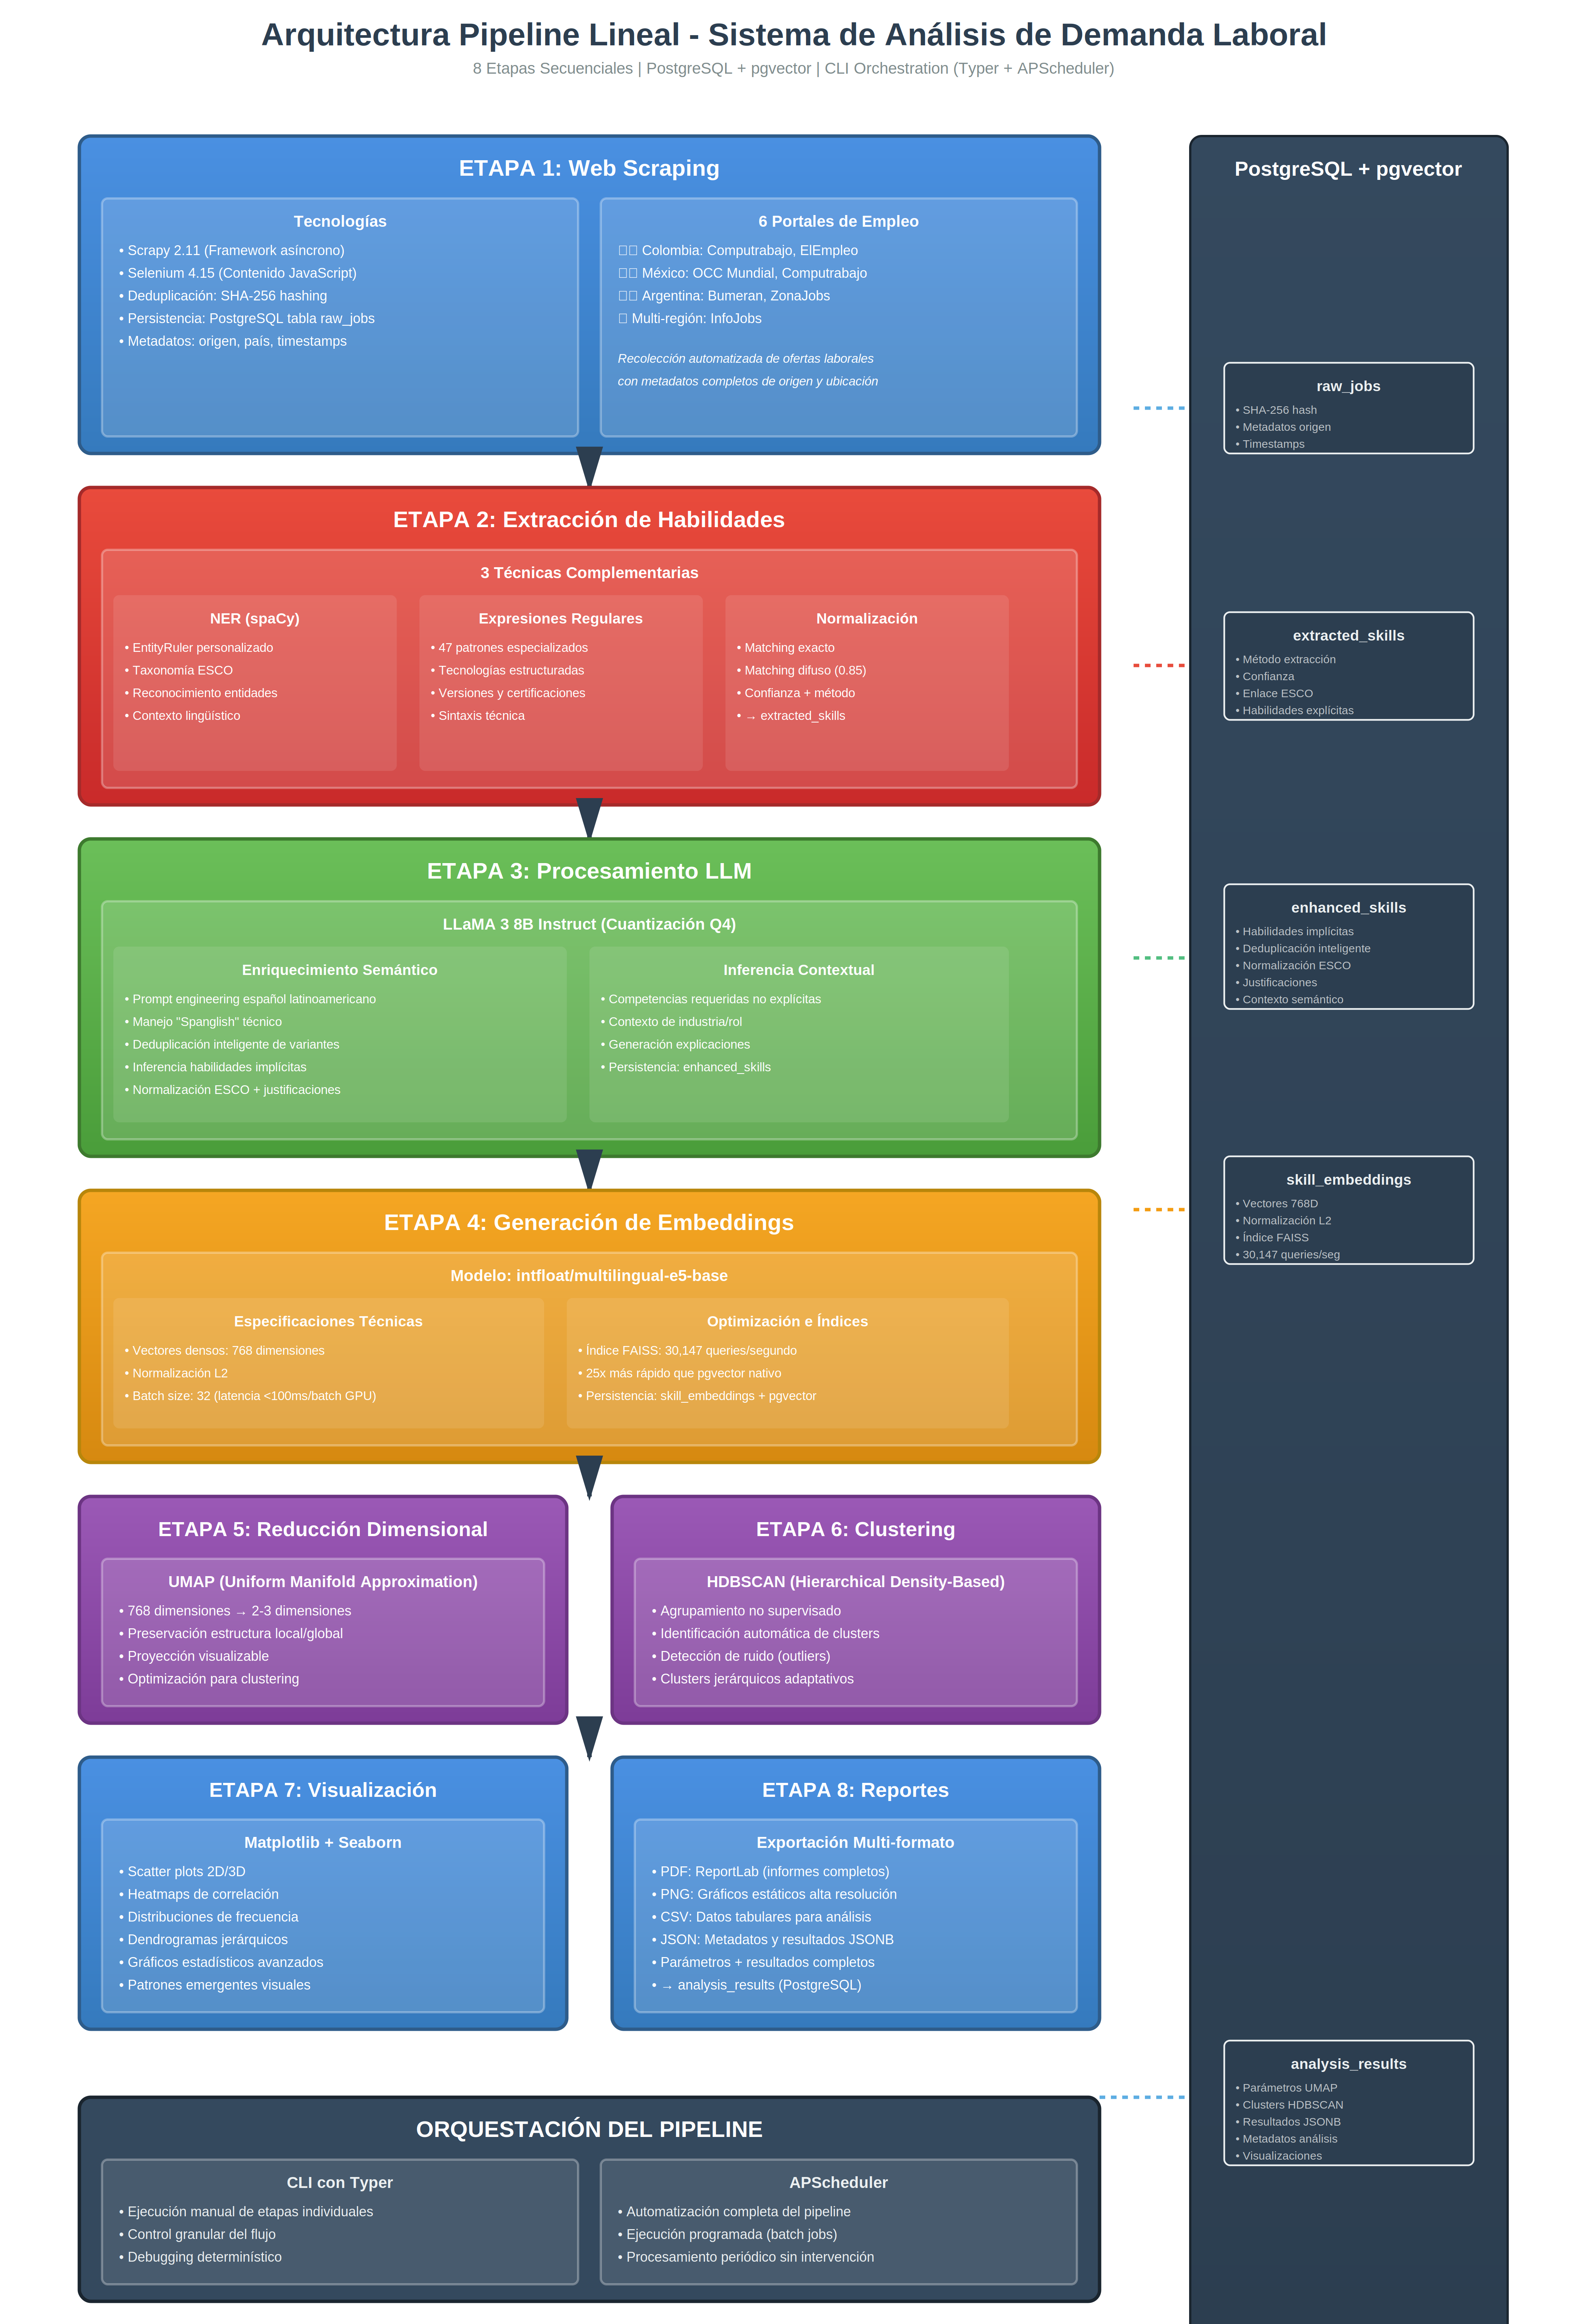
\includegraphics[width=0.85\textwidth]{diagrams/pipeline_arquitectura.png}
\caption{Arquitectura Modular del Observatorio - Pipeline de 8 Etapas}
\label{fig:arquitectura-completa}
\end{figure}

La Figura \ref{fig:arquitectura-completa} presenta la vista modular completa del pipeline, detallando tecnologías específicas, funciones, entradas/salidas y mecanismos de almacenamiento por módulo. Cada módulo puede ejecutarse independientemente con fines de desarrollo y pruebas unitarias.

\subsection{Componentes del Sistema}

En la Figura \ref{fig:arquitectura-completa} se presenta una vista de alto nivel de los componentes principales del sistema. Dicha arquitectura ha sido diseñada considerando principios de modularidad y separación de responsabilidades, permitiendo la trazabilidad completa de las transformaciones de datos. Las ocho etapas del pipeline se agrupan en cinco componentes funcionales que se describen a continuación.

El primer componente corresponde al \textbf{servicio de web scraping}, el cual administra la recolección automatizada de ofertas laborales desde seis portales de empleo en Colombia, México y Argentina (Computrabajo, Bumeran, ElEmpleo, InfoJobs, OCC Mundial, ZonaJobs). Este servicio fue implementado utilizando Scrapy 2.11 como framework asíncrono base, complementado con Selenium 4.15 para el manejo de contenido dinámico JavaScript. La deduplicación de ofertas se realiza mediante hashing SHA-256, almacenando las ofertas únicas en la tabla raw\_jobs con metadatos de origen, país y timestamps.

El segundo componente es el \textbf{servicio de extracción de habilidades}, responsable de identificar las competencias técnicas mencionadas explícitamente en las ofertas laborales. Integra tres técnicas complementarias: Reconocimiento de Entidades Nombradas (NER) con spaCy y EntityRuler poblado con taxonomía ESCO, expresiones regulares con 47 patrones para tecnologías estructuradas, y normalización mediante matching de dos capas (exacto y difuso con threshold 0.85). Los resultados se persisten en la tabla extracted\_skills con metadatos de método, confianza y enlace ESCO.

El tercer componente es el \textbf{servicio de procesamiento con LLM}, diseñado para enriquecimiento semántico e inferencia de habilidades implícitas. Utiliza LLaMA 3 8B Instruct (cuantización Q4) con prompt engineering específico para español latinoamericano, manejando el fenómeno de ``Spanglish'' técnico. Las tareas incluyen deduplicación inteligente de variantes sintácticas, inferencia contextual de competencias requeridas, normalización con ESCO, y generación de justificaciones explicables, persistiendo en la tabla enhanced\_skills.

El cuarto componente es el \textbf{servicio de generación de embeddings}, el cual transforma las habilidades en representaciones vectoriales densas de 768 dimensiones mediante el modelo intfloat/multilingual-e5-base. Genera embeddings por lotes (batch\_size=32, latencia $<$100ms/batch en GPU) con normalización L2, almacenando en la tabla skill\_embeddings con soporte pgvector. La construcción de índice FAISS permite 30,147 queries/segundo, superando 25x la velocidad de pgvector nativo.

El quinto componente es el \textbf{servicio de análisis, visualización y reportes}, responsable del descubrimiento de patrones emergentes mediante técnicas no supervisadas. Integra reducción dimensional con UMAP (768D $\rightarrow$ 2-3D), clustering jerárquico con HDBSCAN (identificación automática de clústeres y detección de ruido), generación de visualizaciones con matplotlib/seaborn (scatter plots, heatmaps, distribuciones), y exportación multi-formato (PDF con ReportLab, PNG, CSV, JSON). Los resultados se persisten en analysis\_results con parámetros y resultados en formato JSONB.

\subsection{Diseño de la Base de Datos}

La base de datos actúa como columna vertebral del sistema, implementando el patrón de persistencia de pipeline donde cada etapa escribe sus resultados en tablas especializadas. Se seleccionó \textbf{PostgreSQL 15+} por su soporte JSON nativo (JSONB) para almacenar metadatos flexibles, extensión pgvector para vectores de alta dimensionalidad, robustez transaccional (ACID), capacidad de particionamiento para escalabilidad, y licencia libre (PostgreSQL License).

\subsubsection{Esquema de Tablas Principales}

El esquema consta de seis tablas principales correspondientes a las etapas del pipeline descritas anteriormente:

\textbf{raw\_jobs}: Almacena ofertas tal como fueron scrapeadas. Campos clave: identificador UUID, portal de origen, código de país (CO/MX/AR), título, descripción, requisitos, hash SHA-256 para deduplicación, y bandera de procesamiento.

\textbf{extracted\_skills}: Contiene habilidades identificadas por NER y expresiones regulares. Incluye identificador UUID, referencia a la oferta laboral, texto de la habilidad extraída, método de extracción (NER, regex o ESCO match), score de confianza (0-1), y enlace a la taxonomía ESCO cuando aplica.

\textbf{enhanced\_skills}: Almacena el enriquecimiento semántico realizado por el modelo LLM. Campos principales: identificador, referencia a la oferta, habilidad normalizada, tipo de habilidad (explícita, implícita o normalizada), URI del concepto ESCO, nivel de confianza del LLM, justificación del razonamiento, y modelo utilizado.

\textbf{skill\_embeddings}: Contiene las representaciones vectoriales de 768 dimensiones. Almacena identificador, texto de la habilidad, vector embedding con soporte pgvector, nombre del modelo, y versión. Incluye índice IVFFlat optimizado para búsquedas de similitud coseno con particionamiento en 100 listas.

\textbf{analysis\_results}: Almacena resultados de clustering y análisis de tendencias. Campos: identificador, tipo de análisis (clustering, trends, profile), país, rango de fechas analizado, parámetros de configuración en formato JSONB, y resultados estructurados con clústeres, etiquetas y métricas.

\textbf{esco\_skills}: Tabla de referencia con la taxonomía ESCO completa. Contiene URI del concepto, etiquetas preferidas en español e inglés, etiquetas alternativas, tipo de habilidad, descripción, y nivel de reutilización. Almacena 13,174 habilidades (13,000 de ESCO v1.1.0 más 174 agregadas manualmente).

\begin{figure}[H]
\centering
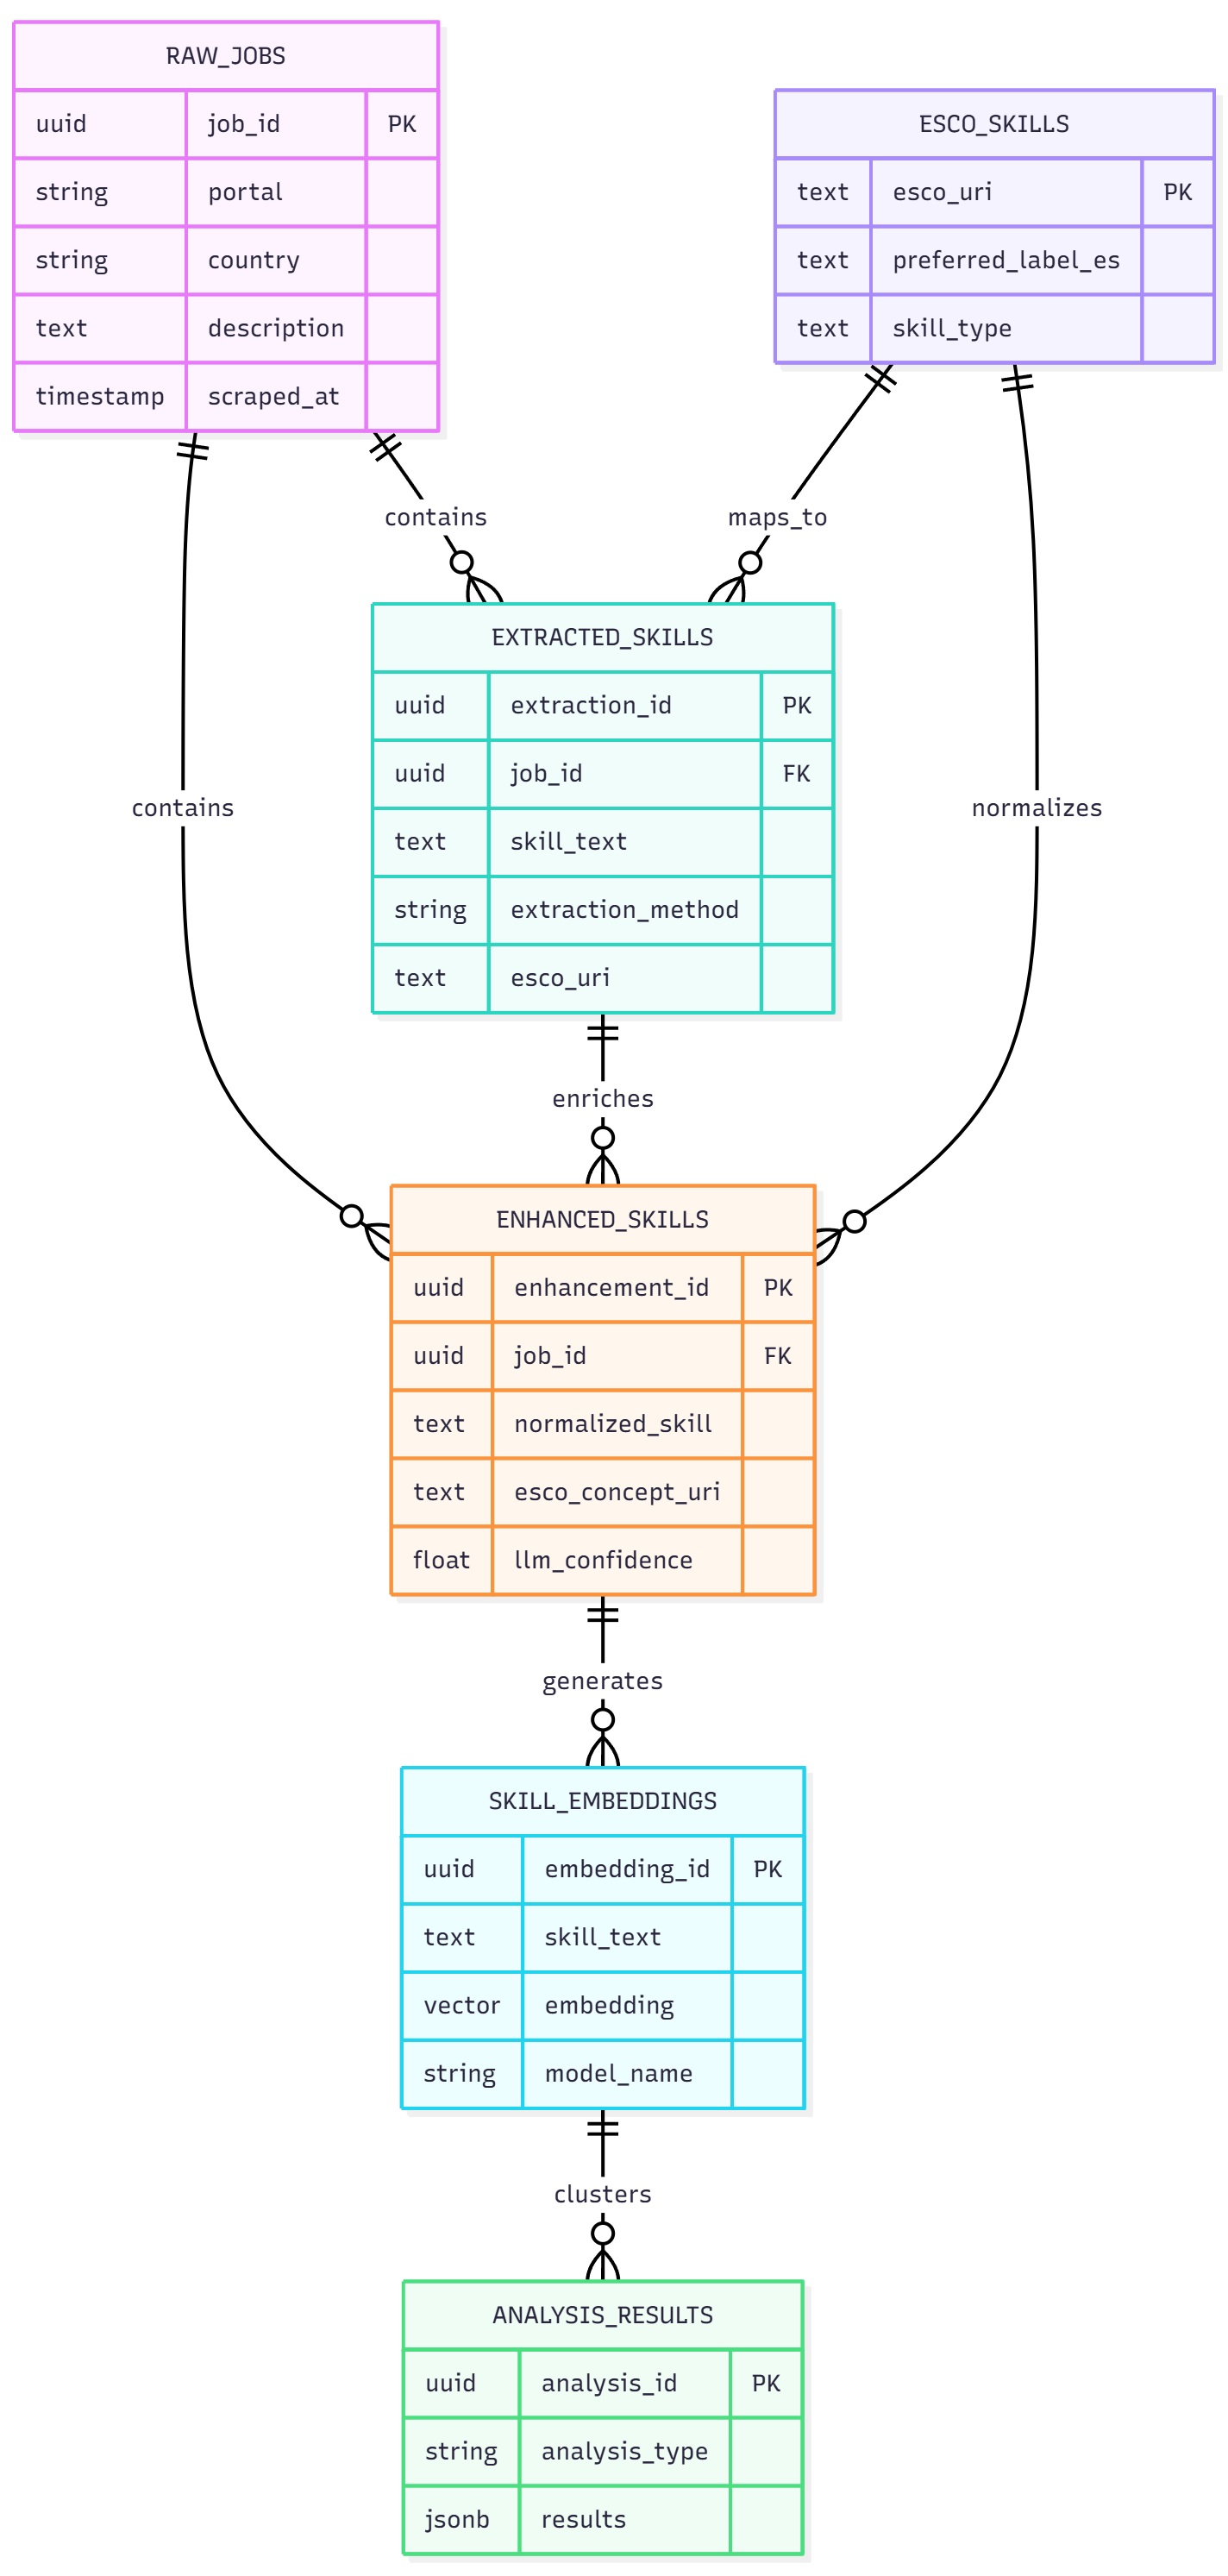
\includegraphics[width=0.5\textwidth]{diagrams/DiagramaER.png}
\caption{Diagrama Entidad-Relación de la Base de Datos}
\label{fig:diagrama-er}
\end{figure}

La Figura \ref{fig:diagrama-er} muestra las relaciones entre tablas. Todas las tablas derivadas mantienen referencia mediante llave foránea hacia la tabla de ofertas laborales (raw\_jobs), garantizando trazabilidad completa desde cualquier resultado de análisis hasta la oferta original. Las tablas de habilidades extraídas y enriquecidas mantienen referencia opcional hacia la taxonomía ESCO para efectos de normalización.

\section{Herramientas y Tecnologías}

Las Tablas \ref{tab:tech-stack-infra} y \ref{tab:tech-stack-analytics} resumen las decisiones tecnológicas fundamentales y su justificación académica y técnica, organizadas por capa funcional del sistema.

\begin{table}[H]
\centering
\caption{Stack Tecnológico: Infraestructura y Adquisición de Datos}
\label{tab:tech-stack-infra}
\begin{tabular}{|p{3.5cm}|p{3.5cm}|p{6.5cm}|}
\hline
\textbf{Componente} & \textbf{Tecnología} & \textbf{Justificación} \\
\hline
Base de datos & PostgreSQL 15+ con pgvector & Soporte JSONB para metadatos flexibles, extensión pgvector para vectores 768D, robustez ACID, particionamiento para escalabilidad. \\
\hline
Taxonomía & ESCO v1.1.0 (+ 174 manuales) & Cobertura 13,000+ skills con etiquetas español/inglés, estructura ontológica con URIs, respaldo institucional CE, licencia CC BY 4.0. \\
\hline
Framework scraping & Scrapy 2.11 + Selenium 4.15 & Arquitectura asíncrona (100+ req/min), manejo robusto de reintentos, middlewares extensibles, Selenium para JavaScript dinámico. \\
\hline
Modelo NLP español & spaCy 3.7 + es\_core\_news\_lg & Mejor modelo español disponible (97M parámetros), soporte EntityRuler para ESCO, optimizado CPU ($<$100ms/doc). \\
\hline
Lenguaje & Python 3.11+ & Ecosistema científico maduro (NumPy, pandas, scikit-learn), bibliotecas NLP referencia (spaCy, transformers), integración PostgreSQL. \\
\hline
Control versiones & Git + GitHub & Estándar industria, integración CI/CD (GitHub Actions), control issues/milestones, documentación Markdown, respaldo cloud. \\
\hline
\end{tabular}
\end{table}

\begin{table}[H]
\centering
\caption{Stack Tecnológico: Procesamiento y Análisis}
\label{tab:tech-stack-analytics}
\begin{tabular}{|p{3.5cm}|p{3.5cm}|p{6.5cm}|}
\hline
\textbf{Componente} & \textbf{Tecnología} & \textbf{Justificación} \\
\hline
LLM enriquecimiento & LLaMA 3 8B Instruct (Q4) & F1=0.64 en español técnico, despliegue local sin APIs (privacidad), cuantización Q4 (8-10 GB VRAM), tokenización eficiente 1.3 tokens/palabra. \\
\hline
Embeddings & intfloat/multilingual-e5-base & Estado del arte multilingüe (768D), contrastive learning en 100 idiomas, normalización L2 integrada, 278M parámetros ejecutables CPU. \\
\hline
Índice similitud & FAISS IndexFlatIP & Velocidad 30,147 q/s (25x superior pgvector), búsqueda exacta (100\% recall), latencia 0.033ms, Facebook AI Research. \\
\hline
Reducción dimensional & UMAP \cite{mcinnes2018umap} & Preserva estructura local y global (superior t-SNE), escalabilidad millones puntos, reproducibilidad con semilla fija, parámetros interpretables. \\
\hline
Clustering & HDBSCAN \cite{campello2013} & No requiere especificar k, identifica ruido automático, maneja densidades variables (nicho vs. mainstream), jerarquía multinivel. \\
\hline
Orquestación & Typer CLI + APScheduler & Interface tipo Git con validación automática, scheduler 24/7, logging estructurado, integración cron/systemd. \\
\hline
\end{tabular}
\end{table}

Todas las tecnologías seleccionadas cumplen con criterios de: (1) Licencias permisivas (MIT, Apache 2.0, PostgreSQL, CC BY) permitiendo uso académico y potencial comercial futuro; (2) Madurez y estabilidad con versiones $\geq$ 2.0 y comunidades activas; (3) Documentación académica completa con publicaciones científicas revisadas por pares para componentes críticos; (4) Reproducibilidad mediante control de versiones de dependencias y semillas fijas para componentes estocásticos; (5) Escalabilidad demostrada para el objetivo de 600,000 ofertas laborales mediante arquitectura de pipeline por lotes y particionamiento de base de datos.
